% ============================================================
%  SICOLEGIO 360 --- Documento Academico Completo
%  Curso: Sistemas de Informacion  |  Ciclo 7
%  Elaborado con LaTeX (clase report)
% ============================================================
\documentclass[12pt,a4paper,oneside]{report}

% -- Paquetes esenciales -------------------------------------
\usepackage[T1]{fontenc}
\usepackage[utf8]{inputenc}
\usepackage[provide=*,spanish]{babel}
\addto\captionsspanish{\renewcommand{\tablename}{Tabla}}
\addto\captionsspanish{\renewcommand{\listtablename}{\'Indice de Tablas}}
\addto\captionsspanish{\renewcommand{\listfigurename}{\'Indice de Figuras}}
\addto\captionsspanish{\renewcommand{\appendixname}{Anexo}}
\addto\captionsspanish{\renewcommand{\contentsname}{\'Indice General}}
\usepackage{lmodern}

% -- Geometria -----------------------------------------------
\usepackage[
  top=2.54cm, bottom=2.54cm,
  left=2.54cm, right=2.54cm,
  headheight=28pt
]{geometry}

% -- Colores -------------------------------------------------
\usepackage[table]{xcolor}
\definecolor{azulOscuro}{RGB}{10,47,97}
\definecolor{azulMedio}{RGB}{28,100,180}
\definecolor{verdInst}{RGB}{34,120,80}
\definecolor{grisClaro}{RGB}{245,246,248}
\definecolor{grisTabla}{RGB}{220,225,232}
\definecolor{dorado}{RGB}{180,140,20}

% -- Tipografia (Times New Roman para APA 7) -----------------
\usepackage{times}

% -- Encabezados y pies (Formato APA 7 sin colores ni lineas) -
\usepackage{fancyhdr}
\pagestyle{fancy}
\fancyhf{}
\fancyhead[L]{\small\MakeUppercase{SICOLEGIO 360: Plataforma Multiinstitucional}}
\fancyhead[R]{\thepage}
\fancyfoot{}
\renewcommand{\headrulewidth}{0pt}

% -- Secciones en formato APA 7 (sin color, sin lineas) -----
\usepackage{titlesec}
\titleformat{\chapter}
  {\normalfont\bfseries\Large\centering}
  {\thechapter\quad}
  {0pt}
  {}
\titlespacing*{\chapter}{0pt}{-25pt}{15pt}
\titleformat{\section}
  {\normalfont\bfseries\large}{\thesection}{1em}{}
\titleformat{\subsection}
  {\normalfont\bfseries\itshape\normalsize}{\thesubsection}{1em}{}
\titleformat{\subsubsection}
  {\normalfont\bfseries\normalsize}{\thesubsubsection}{1em}{}

% -- Listas --------------------------------------------------
\usepackage{enumitem}
\setlist[itemize]{leftmargin=1.5em,itemsep=2pt,topsep=4pt}
\setlist[enumerate]{leftmargin=1.5em,itemsep=2pt,topsep=4pt}

% -- Tablas --------------------------------------------------
\usepackage{booktabs}
\usepackage{longtable}
\usepackage{array}
\usepackage{multirow}
\usepackage{tabularx}
\renewcommand{\arraystretch}{1.35}

% -- Figuras y Captions al estilo APA 7 ----------------------
\usepackage{graphicx}
\usepackage{float}
\usepackage{caption}
\usepackage{subcaption}
\captionsetup[table]{labelfont=bf,textfont=it,labelsep=newline,singlelinecheck=off,justification=raggedright}
\captionsetup[figure]{labelfont=bf,textfont=it,labelsep=newline,singlelinecheck=off,justification=raggedright}

% -- Hiperenlaces (APA: negro para formato impreso/sobrio) ----
\usepackage{hyperref}
\hypersetup{
  colorlinks=true,
  linkcolor=black,
  citecolor=black,
  urlcolor=black,
  pdftitle={SICOLEGIO 360 — Sistema de Información Multiinstitucional},
  pdfauthor={Curso Sistemas de Información},
  pdfsubject={Proyecto académico},
}

% -- Bibliografía (APA: Autor-Año con natbib) ---------------
\usepackage[authoryear]{natbib}
\setcitestyle{authoryear,round,aysep={,}}

% -- Utilidades ----------------------------------------------
\usepackage{amsmath}
\usepackage{amssymb}
\usepackage{tocloft}
\setcounter{tocdepth}{1} % Solo mostrar Capitulos y Secciones en el Indice General
% -- Personalizacion de Tocloft para APA 7 (Centrado y Puntos) --
\renewcommand{\cfttoctitlefont}{\hfill\normalfont\bfseries\Large}
\renewcommand{\cftaftertoctitle}{\hfill}
\renewcommand{\cftlottitlefont}{\hfill\normalfont\bfseries\Large}
\renewcommand{\cftafterlottitle}{\hfill}
\renewcommand{\cftloftitlefont}{\hfill\normalfont\bfseries\Large}
\renewcommand{\cftafterloftitle}{\hfill}
\renewcommand{\cftchapleader}{\cftdotfill{\cftdotsep}} % Habilitar lineas de puntos para capitulos
\setlength{\cftbeforetoctitleskip}{-25pt}
\setlength{\cftaftertoctitleskip}{15pt}
\setlength{\cftbeforelottitleskip}{-25pt}
\setlength{\cftafterlottitleskip}{15pt}
\setlength{\cftbeforeloftitleskip}{-25pt}
\setlength{\cftafterloftitleskip}{15pt}
\usepackage{rotating}
\usepackage{framed}
\usepackage{setspace}

% -- Espaciado y Sangrias APA 7 -----------------------------
\usepackage{indentfirst} % Forzar sangria en el primer parrafo de cada seccion
\setlength{\parskip}{0pt}
\setlength{\parindent}{1.27cm}

% -- Caja destacada ------------------------------------------
\newenvironment{cajaConcepto}[1][]{%
  \begin{framed}\noindent{\bfseries #1}\par\smallskip
}{\end{framed}}

% ═══════════════════
\begin{document}
\sloppy
\doublespacing

% ─────────────────────────────────────────────────────────────
%  PORTADA (Estilo APA 7 - Sin color, fondo blanco y tipografía sobria)
% ─────────────────────────────────────────────────────────────
\begin{titlepage}
    \begin{center}
        \setstretch{1.1}
        {\fontsize{14}{16}\selectfont\textbf{UNIVERSIDAD NACIONAL AGRARIA DE LA SELVA}} \\[0.3cm]
        {\fontsize{13}{15}\selectfont\textbf{FACULTAD DE INGENIERÍA EN INFORMÁTICA Y SISTEMAS}} \\[0.2cm]
        {\fontsize{12}{14}\selectfont\textbf{ESCUELA PROFESIONAL DE INGENIERÍA DE SISTEMAS}} \\[0.4cm]
        
        % Bloques para logos institucionales
        \begin{minipage}{0.45\textwidth}
            \centering
            
\includegraphics[height=8cm,keepaspectratio]{logounas.png}
        \end{minipage}
        \hfill
        \begin{minipage}{0.45\textwidth}
            \centering
            
\includegraphics[height=5cm,keepaspectratio]{LOGO-FIIS-1000x1000-TR.png}
        \end{minipage}\\[0 cm]
        
        % Línea divisoria elegante
        \rule{\linewidth}{1.5pt} \\[0.6cm]
        
        % Título del proyecto
        {\fontsize{13}{16}\selectfont\textbf{DE LAS TRANSACCIONES OPERATIVAS A LA ESTRATEGIA GERENCIAL: ANÁLISIS DE DATOS PARA LA TOMA DE DECISIONES EN SICOLEGIO 360}} \\[0.6cm]
        
        \rule{\linewidth}{1.5pt} \\[1.5cm]
        
        % Información del curso y autores
        \setstretch{1.5}
        \begin{minipage}{0.85\textwidth}
            \begin{flushleft}
                \begin{tabular}{@{}p{3.5cm}p{9.5cm}@{}}
                    \textbf{Curso:} & Sistemas de Información \\[0.2cm]
                    \textbf{Autores:} & Evaristo Jara, Jose Junior \\
                                      & Tapullima Serna, Meselemias \\[0.2cm]
                    \textbf{Docente:} & Docente del Curso \\[0.2cm]
                    \textbf{Ciclo:} & Séptimo \\[0.2cm]
                \end{tabular}
            \end{flushleft}
        \end{minipage}
        
        \vfill
        
        % Ubicación y Fecha
        {\fontsize{12}{14}\selectfont\textbf{Tingo María -- Perú}} \\[0.2cm]
        {\fontsize{12}{14}\selectfont\textbf{2026}}
    \end{center}
\end{titlepage}

% ─────────────────────────────────────────────────────────────
%  RESUMEN
% ─────────────────────────────────────────────────────────────
\chapter*{Resumen}
\addcontentsline{toc}{chapter}{Resumen}
\markboth{RESUMEN}{RESUMEN}

El presente trabajo académico propone el diseño de \textbf{SICOLEGIO 360}, una plataforma multiinstitucional de sistema de información con enfoque socio-tecnológico, orientada a mejorar la gestión académica, administrativa, financiera y comunicacional de instituciones educativas privadas de nivel básico regular en el Perú y América Latina.

La problemática identificada parte del diagnóstico de que gran parte de los colegios privados pequeños y medianos continúan gestionando sus procesos mediante registros manuales, hojas de cálculo desconectadas, archivos físicos y canales informales de comunicación como WhatsApp. Esto genera pérdida de información, duplicidad de registros, demoras en los reportes, errores en el cálculo de notas y promedios, descontrol en los pagos de pensiones y una comunicación deficiente con los padres de familia.

Frente a esta realidad, SICOLEGIO 360 se propone como una solución integral que integra tecnología, organización, personas y procesos bajo el marco del enfoque socio-tecnológico. El sistema trabaja en cuatro niveles organizacionales: operativo, de conocimiento, administrativo y estratégico, aplicando los conceptos de TPS, KWS, MIS, DSS y ESS según las necesidades de cada tipo de usuario, configurando de esta manera las bases de datos transaccionales para garantizar las propiedades ACID en su operatividad diaria.

El documento se estructura en cuatro capítulos principales: el Capítulo I introduce el contexto escolar, el enfoque socio-tecnológico y el diagnóstico detallado de las transacciones manuales; el Capítulo II desarrolla el marco teórico de los sistemas de información, la aplicación de los tipos de sistemas (KWS, MIS, DSS, ESS) y las funciones del TPS dentro de la pirámide organizacional; el Capítulo III detalla el diseño lógico del TPS con sus 21 transacciones operativas, los requerimientos, casos de uso y el diseño de la base de datos relacional de 26 tablas con su diccionario de datos; y el Capítulo IV aborda la ingeniería del software, flujo automatizado, seguridad transaccional, plan de pruebas y los estudios de viabilidad y beneficios.

\textbf{Palabras clave:} sistema de información, plataforma multiinstitucional, gestión académica, enfoque socio-tecnológico, TPS, MIS, DSS, ESS, base de datos relacional, propiedades ACID.

% ─────────────────────────────────────────────────────────────
%  ABSTRACT
% ─────────────────────────────────────────────────────────────
\chapter*{Abstract}
\addcontentsline{toc}{chapter}{Abstract}
\markboth{ABSTRACT}{ABSTRACT}

This academic paper proposes the design of \textbf{SICOLEGIO 360}, a multi-institutional information system platform with a socio-technological approach, aimed at improving the academic, administrative, financial, and communication management of private educational institutions at the basic regular level in Peru and Latin America.

The identified problem stems from the diagnosis that most small and medium private schools continue to manage their processes through manual records, disconnected spreadsheets, physical files, and informal communication channels such as WhatsApp. This generates information loss, duplicate records, delays in reporting, errors in grade and average calculation, poor control over tuition payments, and deficient communication with parents.

In response to this reality, SICOLEGIO 360 is proposed as a comprehensive solution that integrates technology, organization, people, and processes under the socio-technological approach framework. The system operates at four organizational levels: operational, knowledge, administrative, and strategic, applying the concepts of TPS, KWS, MIS, DSS, and ESS according to each type of user's needs, establishing a transactional database backend to ensure ACID properties in daily operations.

The document is organized into four core chapters: Chapter I introduces the school context, socio-technological approach, and the detailed diagnosis of manual processes; Chapter II details the theoretical framework of information systems, the application of various system types (KWS, MIS, DSS, ESS), and TPS functions within the organizational pyramid; Chapter III presents the logical design of the TPS, including its 21 transactions, requirements, use cases, and the 26-table relational database structure with data dictionaries; and Chapter IV discusses software engineering, automated workflows, transactional security, test plans, and overall feasibility and benefits.

\textbf{Keywords:} information system, multi-institutional platform, academic management, socio-technological approach, TPS, MIS, DSS, ESS, relational database, ACID properties.

% ─────────────────────────────────────────────────────────────
%  ÍNDICES
% ─────────────────────────────────────────────────────────────
\newpage 
\tableofcontents
\newpage
\listoftables
\newpage
\listoffigures

% ─────────────────────────────────────────────────────────────
%  INTRODUCCIÓN
% ─────────────────────────────────────────────────────────────
\chapter*{Introducción}
\addcontentsline{toc}{chapter}{Introducción}
\markboth{INTRODUCCIÓN}{INTRODUCCIÓN}

La educación es uno de los servicios más importantes que una sociedad puede ofrecer a sus ciudadanos. Sin embargo, en un contexto donde la tecnología ha transformado casi todas las industrias, muchas instituciones educativas privadas pequeñas y medianas aún operan con métodos administrativos y académicos tradicionales: cuadernos de asistencia, libretas físicas, recibos de pago manuales y comunicaciones dispersas a través de mensajes de WhatsApp.

Esta brecha tecnológica no es un problema menor. Cuando la información de un colegio está fragmentada en distintos archivos, cuadernos y personas, el riesgo de error es alto, la toma de decisiones se vuelve lenta e imprecisa, y la experiencia de padres, estudiantes y docentes se deteriora progresivamente. El núcleo de este problema radica en la ineficiencia con la que se procesan las transacciones cotidianas de la organización.

El presente trabajo académico propone el diseño de \textbf{SICOLEGIO 360}, una plataforma multiinstitucional concebida como un \textbf{Sistema de Procesamiento de Transacciones (TPS)} con enfoque socio-tecnológico. El sistema permite a varios colegios gestionar de manera integrada y consistente sus transacciones académicas, administrativas, financieras y comunicacionales desde una única base de datos, garantizando que cada registro se almacene de forma aislada, consistente y segura.

El informe está organizado en cuatro capítulos principales:
\begin{itemize}
    \item \textbf{Capítulo I: La Organización y el Diagnóstico de Procesos Manuales}, donde se describe a las instituciones escolares, se plantea el enfoque socio-tecnológico y se detalla el flujo operativo y problemático antes de la automatización.
    \item \textbf{Capítulo II: Marco Teórico y Enfoque de Sistemas Transaccionales (TPS)}, que recopila los fundamentos de los sistemas de información, la aplicación profunda de los tipos de sistemas (KWS, MIS, DSS, ESS), el mapeo en la pirámide organizacional, los indicadores del sistema y la teoría de consistencia transaccional ACID.
    \item \textbf{Capítulo III: Propuesta y Diseño Lógico del TPS SICOLEGIO 360}, que detalla el diseño de tres capas, el catálogo de macro-módulos y el módulo jerárquico de IE, la matriz de las 21 transacciones operativas del sistema, requerimientos de software y el modelo de datos relacional de 26 tablas con sus diccionarios de datos.
    \item \textbf{Capítulo IV: Ingeniería, Implementación, Beneficios y Viabilidad del TPS}, donde se expone la configuración práctica del entorno de desarrollo, la estructura de archivos, el control de seguridad y código transaccional SQL, el plan de pruebas, la matriz de beneficios por actor, y el análisis de viabilidades.
\end{itemize}

Este documento busca aplicar de manera práctica los conceptos del curso de Sistemas de Información, proyectando una solución real, útil y altamente transaccional para el sector educativo escolar.

% ═══════════════════════════════════════════════════════════════
%  CAPÍTULO I: LA ORGANIZACIÓN Y EL DIAGNÓSTICO DE PROCESOS MANUALES
% ═══════════════════════════════════════════════════════════════
\chapter{La Organización y el Diagnóstico de Procesos Manuales}

\section{Contexto de la organización escolar}

\subsection{Las instituciones educativas privadas como organizaciones de servicios}
Las instituciones educativas privadas son organizaciones dedicadas a la prestación de un servicio social y formativo de nivel básico regular. A diferencia de las industrias que producen bienes tangibles, los colegios generan valor a través de la formación académica, el desarrollo de competencias y el acompañamiento familiar. Desde la perspectiva de los sistemas de información, un colegio representa una organización de servicios compleja que maneja una densa red de datos operativos interrelacionados.

La gestión de la información en estas organizaciones no es un aspecto complementario, sino la base que sustenta la sostenibilidad operativa y la calidad del servicio. Un colegio requiere registrar y procesar diariamente un alto volumen de eventos transaccionales relacionados con sus estudiantes, docentes, notas, asistencias, justificaciones, pagos y comunicaciones.

\subsection{Tipos de organizaciones y roles del sistema}
SICOLEGIO 360 se dirige a instituciones educativas privadas pequeñas y medianas del nivel básico regular (inicial, primaria y secundaria), caracterizadas por:
\begin{itemize}
    \item \textbf{Colegios privados pequeños:} Con una población menor a 200 estudiantes y una estructura administrativa mínima, donde el personal suele cumplir múltiples roles (secretaría y tesorería simultáneamente).
    \item \textbf{Colegios privados medianos:} Con una población de 200 a 800 estudiantes, áreas funcionales diferenciadas y un volumen considerable de transacciones operativas diarias.
\end{itemize}
Los actores involucrados en la ejecución de transacciones dentro de esta organización incluyen al \textit{Superadministrador de la plataforma} (gestor del negocio SaaS), el \textit{Administrador del colegio} (configurador de la base académica), el \textit{Director} (usuario estratégico), el \textit{Docente} (registrador de transacciones académicas), la \textit{Secretaría/Tesorería} (procesadores administrativos y financieros), los \textit{Padres de Familia} y los \textit{Estudiantes} (receptores y consultores autorizados).

\section{El enfoque socio-tecnológico en SICOLEGIO 360}

El diseño de SICOLEGIO 360 adopta un enfoque socio-tecnológico, reconociendo que el éxito del sistema de información depende del ajuste óptimo entre dos dimensiones críticas: la dimensión técnica (el software transaccional, la base de datos relacional) y la dimensión social (el personal de secretaría, los docentes, los padres y los directivos) \citep{laudon2016}.

En este contexto, la introducción de un TPS automatizado ayuda a aplanar la estructura jerárquica del colegio. Al descentralizar el ingreso de datos en la fuente (el docente registra la nota directamente desde su dispositivo y el padre paga mediante la pasarela), se eliminan los intermediarios (coordinadores y secretarias transcribiendo información), lo que agiliza el flujo transaccional y reduce significativamente los costos administrativos.

Como se detalla en el anexo correspondiente, las dimensiones del enfoque socio-tecnológico de SICOLEGIO 360 se estructuran para armonizar el factor social con el técnico, permitiendo que la capacitación y la cultura organizacional jueguen un rol fundamental.

\section{Diagnóstico de los procesos manuales actuales}

En los colegios que no disponen de una plataforma integrada, los flujos administrativos y académicos se caracterizan por una alta dependencia del papel y herramientas de escritorio locales aisladas, lo que da lugar a una gestión fragmentada y vulnerable.

\subsection{Gestión y Registro Administrativo Manual}

\paragraph{Proceso manual de matrícula.} El proceso de matrícula en un colegio sin sistema de información integrado implica la atención presencial del padre de familia en secretaría, el llenado manual de una ficha de matrícula en papel o en un archivo de Excel no compartido, la verificación manual de los datos del estudiante, la asignación manual del grado y la sección, la firma del compromiso de pago en un documento físico y el archivado del expediente en una carpeta física. Este proceso es lento, propenso a errores de transcripción y difícil de consultar posteriormente.

\paragraph{Proceso manual de registro de estudiantes.} El registro de estudiantes se realiza en una hoja de cálculo o en un cuaderno. Cada secretaria tiene su propio formato, lo que genera inconsistencias. Cuando se necesita actualizar un dato del estudiante, debe buscarse el registro en el archivo correspondiente y modificarlo manualmente, con el riesgo de que existan versiones distintas del mismo registro en distintos archivos.

\paragraph{Proceso manual de registro de docentes.} El registro de docentes se realiza de manera similar al de estudiantes: en archivos de Excel o en documentos físicos. La información sobre los cursos asignados a cada docente se maneja por separado, generalmente en un cuadro elaborado manualmente al inicio de cada año escolar.

\paragraph{Proceso manual de asignación de cursos y secciones.} La asignación de cursos y secciones se realiza manualmente, generalmente en una hoja de cálculo o en un cuadro impreso. Este proceso es laborioso y propenso a errores, especialmente cuando hay cambios en la planta docente o en la organización de las secciones.

\subsection{Gestión Académica y Evaluación Manual}

\paragraph{Proceso manual de asistencia.} El control de asistencia se realiza mediante listas impresas que el docente llena a mano al inicio de cada clase. Al final del día, la secretaría debe consolidar las listas de todos los docentes para tener un registro de la asistencia diaria de la institución. Este proceso es lento, propenso a errores y difícil de consultar para períodos anteriores.

\paragraph{Proceso manual de registro de notas.} Las notas son registradas por los docentes en sus cuadernos personales o en archivos de Excel individuales. Al final del período académico, cada docente entrega sus notas a la secretaría, que las transcribe en un registro centralizado. Este proceso de transcripción es una fuente frecuente de errores.

\paragraph{Proceso manual de cálculo de promedios.} El cálculo de promedios se realiza manualmente por cada docente o por la secretaría académica, aplicando las fórmulas establecidas por la institución. Cuando hay errores en los datos de entrada, los promedios calculados también son incorrectos. Además, la revisión de los cálculos es tediosa y requiere tiempo adicional.

\paragraph{Proceso manual de emisión de libretas.} La elaboración de las libretas de notas es uno de los procesos más laboriosos. La secretaría debe recopilar las notas de todos los cursos de cada estudiante, calcular los promedios, verificar las asistencias y elaborar el documento final. Este proceso puede tomar varios días y es común que se detecten errores después de entregar las libretas a los padres.

\subsection{Gestión Disciplinaria y de Bienestar Manual}

\paragraph{Proceso manual de conducta e incidencias.} Los registros de conducta e incidencias se anotan en cuadernos de incidencias o en informes físicos. Cada docente o tutor maneja su propio registro, lo que hace difícil tener una visión integral del comportamiento de un estudiante a lo largo del tiempo o identificar patrones conductuales en una sección.

\paragraph{Proceso manual de citaciones a padres.} Las citaciones a los padres de familia se realizan por escrito (comunicados físicos enviados con el estudiante), por llamadas telefónicas o por mensajes de WhatsApp. No existe un registro formal de las citaciones realizadas, las respuestas de los padres ni los acuerdos alcanzados en las reuniones.

\subsection{Gestión Financiera, de Comunicados y Alertas Manual}

\paragraph{Proceso manual de pagos de pensiones.} Los pagos de pensiones se registran en recibos físicos numerados y en un cuaderno de control de tesorería. La verificación del estado de pago de un estudiante requiere revisar físicamente los recibos o el cuaderno, lo que es lento e impreciso cuando hay un gran número de estudiantes.

\paragraph{Proceso manual de comunicados escolares.} Los comunicados escolares se envían principalmente de dos maneras: mediante documentos físicos entregados a los estudiantes (que no siempre llegan a los padres) o a través de grupos de WhatsApp (que no garantizan que todos los padres reciban y lean el comunicado). No hay un registro formal de los comunicados enviados ni confirmación de recepción.

\section{Análisis de deficiencias y limitaciones de la gestión manual}

La dependencia de soportes físicos y registros aislados para estas transacciones operativas diarias genera graves deficiencias organizacionales. La Tabla~\ref{tab:problemas} resume de forma detallada los principales problemas detectados y su nivel de impacto en el colegio.

\begin{table}[H]
\centering
\caption{Principales problemas detectados en los procesos manuales}
\label{tab:problemas}
\begin{tabularx}{\textwidth}{lXl}
\toprule
Proceso & Problema principal & Impacto \\
\midrule
Matrícula & Datos incompletos, archivos desactualizados & Alto \\
Registro de notas & Errores de transcripción & Alto \\
Cálculo de promedios & Errores en fórmulas manuales & Alto \\
Emisión de libretas & Demoras y errores & Alto \\
Control de pagos & Pérdida de recibos, datos inconsistentes & Alto \\
Asistencia & Consolidación lenta, datos incompletos & Medio \\
Conducta & Sin registro histórico integrado & Medio \\
Comunicados & Sin confirmación de recepción & Medio \\
Citaciones & Sin registro formal de acuerdos & Medio \\
Reportes & Elaboración manual lenta y laboriosa & Alto \\
\bottomrule
\end{tabularx}
\end{table}

\section{Formulación del problema y objetivos del proyecto}

\subsection{Formulación del problema}
¿De qué manera el diseño de una plataforma multiinstitucional estructurada como un \textbf{Sistema de Procesamiento de Transacciones (TPS)} con enfoque socio-tecnológico puede mejorar la integridad, la velocidad y la consistencia en la gestión académica, administrativa y financiera de las instituciones educativas privadas?

\subsection{Objetivos del proyecto}

\paragraph{Objetivo general:}
Diseñar una plataforma multiinstitucional concebida como un Sistema de Procesamiento de Transacciones (TPS) con enfoque socio-tecnológico para asegurar la consistencia, velocidad y fiabilidad operativa en los colegios privados.

\paragraph{Objetivos específicos:}
\begin{enumerate}
    \item Analizar y estructurar la secuencia de transacciones operativas diarias que ejecutan los colegios en sus dimensiones académica, administrativa y de caja.
    \item Desarrollar una matriz de transacciones que defina con precisión las entradas, los procesos y las salidas de cada evento operativo del sistema.
    \item Diseñar una base de datos relacional robusta bajo un modelo multiinstitucional que separe físicamente las transacciones de cada colegio y garantice las propiedades ACID.
    \item Estructurar requerimientos de software y casos de uso orientados a la consistencia del flujo transaccional.
    \item Diseñar la arquitectura tecnológica de tres capas y las guías de implementación necesarias para la seguridad e integridad del TPS.
\end{enumerate}

% ═══════════════════════════════════════════════════════════════
%  CAPÍTULO II: MARCO TEÓRICO Y ENFOQUE DE SISTEMAS TRANSACCIONALES
% ═══════════════════════════════════════════════════════════════
\chapter{Marco Teórico y Enfoque de Sistemas Transaccionales (TPS)}

\section{Teoría general de los sistemas de información}

Un sistema de información (SI) es un conjunto de componentes interrelacionados que recopilan (o recuperan), procesan, almacenan y distribuyen información para apoyar los procesos de toma de decisiones, coordinación y control en una organización \citep{laudon2016}. Los componentes de entrada, procesamiento, salida y retroalimentación interactúan para transformar datos brutos en información valiosa. Como se muestra en los anexos, este flujo transforma los datos operativos en el insumo esencial para la organización.

Los SI permiten centralizar la información, reducir la redundancia y optimizar el tiempo dedicado a actividades repetitivas en las empresas modernas \citep{obrien2009}.

\section{Aplicación de los tipos de sistemas en SICOLEGIO 360}

Dentro de SICOLEGIO 360 se configuran e implementan diferentes tipos de sistemas de información para dar soporte a cada uno de los niveles organizacionales, desde los flujos puramente operativos hasta la dirección general.

\subsection{Sistemas de Procesamiento de Transacciones (TPS)}
Los TPS de SICOLEGIO 360 registran todas las transacciones operativas diarias de los colegios: matrículas, asistencias, notas, pagos, comunicados e incidencias. Son el cimiento del sistema y la fuente de todos los datos que alimentan los reportes y análisis de niveles superiores. Los usuarios principales de los TPS son la secretaría académica, los docentes y el personal de tesorería.

\subsection{Aplicación de sistemas de oficina en SICOLEGIO 360}
Los sistemas de oficina en SICOLEGIO 360 apoyan las tareas documentarias del personal administrativo y docente. Incluyen la generación automática de documentos como constancias de estudios, constancias de matrícula, libretas de notas, reportes de asistencia y comunicados institucionales. Estos documentos se generan en formatos estándar (PDF) y pueden personalizarse con el logo y los colores de cada institución.

\subsection{Aplicación de KWS en SICOLEGIO 360}
Los sistemas de trabajo de conocimiento en SICOLEGIO 360 apoyan a los docentes, coordinadores y tutores en su trabajo de análisis y planificación académica. Incluyen herramientas para el análisis del rendimiento por sección, la identificación de estudiantes que necesitan apoyo adicional, el diseño de estrategias de intervención y el seguimiento de los resultados de las acciones tomadas.

\subsection{Aplicación de MIS en SICOLEGIO 360}
El nivel MIS de SICOLEGIO 360 genera reportes periódicos para los coordinadores y directores de los colegios. Los reportes incluyen: promedio académico por grado y sección, porcentaje de asistencia por sección, tasa de morosidad por mes, número de incidencias conductuales por período, estado de matrículas y evolución del rendimiento académico. Estos reportes permiten a los gerentes educativos monitorear el desempeño institucional y tomar decisiones de control.

\subsection{Aplicación de DSS en SICOLEGIO 360}
El nivel DSS de SICOLEGIO 360 apoya la toma de decisiones semiestructuradas de los directivos. Permite analizar datos desde múltiples perspectivas: comparar el rendimiento de diferentes secciones, identificar correlaciones entre asistencia y rendimiento académico, analizar la evolución de la morosidad a lo largo del año y proyectar el comportamiento de matrícula para el siguiente período. El director puede formular preguntas interactivas al sistema y obtener respuestas basadas en los datos disponibles.

\subsection{Aplicación de ESS/EIS en SICOLEGIO 360}
El nivel ESS de SICOLEGIO 360 está orientado al superadministrador de la plataforma y a los promotores o dueños de los colegios. Proporciona una vista global del desempeño de la plataforma y de cada institución: número de colegios registrados, número de estudiantes gestionados, ingresos generados, crecimiento histórico, tendencias de uso y proyecciones de expansión. La información se presenta en tableros de control con gráficos y medidores de desempeño.

\subsection{Relación entre los sistemas dentro de SICOLEGIO 360}
Los distintos tipos de sistemas de SICOLEGIO 360 están interconectados y se alimentan mutuamente. Los datos registrados por los TPS son consolidados por el MIS para generar reportes de control. El DSS utiliza esos reportes para apoyar el análisis y la toma de decisiones. El ESS recibe información de todos los niveles para proporcionar una visión estratégica de la plataforma y de cada institución.

\subsection{Flujo de información desde el nivel operativo hasta el nivel estratégico}
La información en SICOLEGIO 360 fluye de manera ascendente: las transacciones operativas (TPS) generan datos que son procesados y consolidados en reportes gerenciales (MIS), que a su vez alimentan el análisis para la toma de decisiones (DSS) y la visión estratégica de la alta dirección (ESS). Este flujo garantiza que los tomadores de decisiones en todos los niveles tengan acceso a la información que necesitan, en el formato y la oportunidad adecuados.

\section{Funciones del sistema en la pirámide organizacional}

\subsection{Niveles organizacionales y sistemas de información}
Las organizaciones tienen cuatro niveles: operativo, de conocimiento, administrativo y estratégico. Cada nivel tiene necesidades de información diferentes, y los sistemas de información deben diseñarse para satisfacer esas necesidades específicas. SICOLEGIO 360 opera en los cuatro niveles, proporcionando a cada tipo de usuario la información que necesita para realizar su trabajo.

\subsection{Nivel operativo: TPS}
En el nivel operativo, SICOLEGIO 360 actúa como un sistema de procesamiento de transacciones (TPS) que registra todas las operaciones diarias del colegio. Los usuarios principales de este nivel son la secretaría académica, los docentes y el personal de tesorería. Las transacciones incluyen matrícula, asistencia, notas, pagos y comunicados.

\subsection{Nivel del conocimiento: KWS y sistemas de oficina}
En el nivel de conocimiento, SICOLEGIO 360 proporciona herramientas para que los docentes, tutores y coordinadores analicen la información disponible, generen documentos y tomen decisiones informadas sobre la gestión de sus aulas. Las herramientas incluyen reportes de rendimiento por sección, generación de libretas, análisis de asistencia y comunicación con padres.

\subsection{Nivel administrativo: MIS y DSS}
En el nivel administrativo, SICOLEGIO 360 genera reportes gerenciales (MIS) y apoya el análisis para la toma de decisiones (DSS). Los usuarios de este nivel son los directores, coordinadores y administradores de los colegios. Los reportes incluyen estadísticas de rendimiento, asistencia, conducta y finanzas.

\subsection{Nivel estratégico: ESS/EIS}
En el nivel estratégico, SICOLEGIO 360 proporciona tableros de control e indicadores globales para el superadministrador de la plataforma y los promotores de los colegios. La información incluye tendencias de crecimiento, proyecciones de matrícula y desempeño global de la plataforma.

\subsection{Usuarios atendidos por cada nivel de la pirámide}
La Tabla~\ref{tab:usuarios} estructura formalmente los perfiles de usuario que interactúan con cada uno de los niveles de sistemas de información dentro del ecosistema del colegio.

\begin{table}[H]
\centering
\caption{Usuarios por nivel de sistema en SICOLEGIO 360}
\label{tab:usuarios}
\begin{tabularx}{\textwidth}{llX}
\toprule
Nivel & Sistema & Usuarios \\
\midrule
Operativo & TPS & Secretaría, docentes, tesorería \\
Conocimiento & KWS, Office & Docentes, tutores, coordinadores \\
Administrativo & MIS, DSS & Directores, coordinadores, administradores \\
Estratégico & ESS/EIS & Superadmin, promotores, directivos generales \\
\bottomrule
\end{tabularx}
\end{table}

\section{El TPS como base organizacional y garantías ACID}

\subsection{Importancia de los TPS en SICOLEGIO 360}
Los TPS de SICOLEGIO 360 permiten registrar las operaciones diarias de los colegios, convirtiendo los datos operativos en información útil para reportes, análisis y toma de decisiones. Sin los TPS, los sistemas de niveles superiores (MIS, DSS, ESS) no tendrían datos con los cuales trabajar.

\subsection{Garantías del TPS: Propiedades ACID}
Para que un TPS sea considerado fiable y robusto, el motor de base de datos relacional que lo soporta debe implementar las propiedades ACID:
\begin{itemize}
    \item \textbf{Atomicidad (Atomicity):} Asegura que la transacción se ejecute por completo o no se ejecute en absoluto. Por ejemplo, al registrar una matrícula, el sistema guarda los datos del estudiante y el primer cobro de pensión asociados; si falla el guardado de la pensión, la creación del estudiante se revierte automáticamente para evitar registros parciales o fantasmas.
    \item \textbf{Consistencia (Consistency):} Garantiza que una transacción lleve la base de datos de un estado válido a otro. Las reglas de integridad del negocio (ej. no permitir registrar notas superiores a 20 o registrar una asistencia para un curso inexistente) se cumplen estrictamente.
    \item \textbf{Aislamiento (Isolation):} Asegura que las transacciones ejecutadas simultáneamente no interfieran entre sí. Si dos secretarias intentan matricular estudiantes asignándolos a la última vacante disponible de una sección al mismo tiempo, el sistema las procesará secuencialmente, otorgando la vacante a la primera y notificando la falta de cupo a la segunda.
    \item \textbf{Durabilidad (Durability):} Garantiza que una vez que la transacción ha sido completada y guardada, sus efectos persistirán en el almacenamiento físico, incluso si ocurre una falla eléctrica o caída inmediata del servidor.
\end{itemize}

\section{Análisis de datos e indicadores organizacionales}

El sistema captura y procesa múltiples tipos de datos agrupados por dimensiones operativas, calculando indicadores de valor para la gestión.

\subsection{Dimensiones de Datos Analizados}

\paragraph{Datos institucionales.} El sistema analiza datos relacionados con la estructura y el desempeño general de cada institución educativa: número de colegios registrados en la plataforma, número de estudiantes por colegio, número de docentes por institución, niveles educativos activos, crecimiento de matrículas entre períodos y tasa de retención estudiantil.

\paragraph{Datos académicos.} El sistema analiza el rendimiento académico desde múltiples dimensiones: notas promedio por curso, por grado y por sección; porcentaje de estudiantes aprobados y desaprobados por área; evolución del rendimiento a lo largo del período; cursos con mayor tasa de desaprobación; estudiantes con bajo rendimiento en múltiples áreas; y comparación del rendimiento entre secciones del mismo grado.

\paragraph{Datos de asistencia.} El sistema analiza los patrones de asistencia: porcentaje de asistencia por estudiante, por sección y por institución; número de faltas, tardanzas y justificaciones por período; estudiantes con inasistencias frecuentes; días con mayor ausentismo; y correlación entre inasistencia y rendimiento académico.

\paragraph{Datos de conducta.} El sistema analiza los datos de comportamiento estudiantil: número de incidencias por estudiante y por sección; tipos de faltas más frecuentes; estudiantes con incidencias reiteradas; evolución de los problemas conductuales a lo largo del período; y efectividad de las intervenciones realizadas.

\paragraph{Datos financieros.} El sistema analiza el estado financiero del colegio: pagos de matrícula y pensiones recibidos por período; deudas pendientes acumuladas; índice de morosidad; familias con más de dos meses de deuda; ingresos mensuales proyectados vs. recibidos; y comparación de la recaudación entre períodos.

\paragraph{Datos de comunicación con padres.} El sistema analiza la participación de los padres de familia: número de comunicados enviados y leídos; porcentaje de padres que responden a las citaciones; acuerdos registrados y cumplidos; y nivel de participación de los padres en las actividades institucionales.

\subsection{Indicadores principales del sistema}
La Tabla~\ref{tab:indicadores} lista los indicadores más importantes que calcula la plataforma de manera dinámica.

\begin{table}[H]
\centering
\caption{Indicadores principales de SICOLEGIO 360}
\label{tab:indicadores}
\begin{tabularx}{\textwidth}{lXl}
\toprule
Indicador & Qué mide & Nivel \\
\midrule
Tasa de matrícula & Crecimiento de estudiantes registrados & Operativo \\
Promedio académico general & Rendimiento global del estudiante o colegio & Administrativo \\
Porcentaje de asistencia & Participación y permanencia escolar & Operativo \\
Tasa de tardanzas & Puntualidad estudiantil & Operativo \\
Tasa de desaprobación & Cursos o grados con bajo rendimiento & Administrativo \\
Índice de morosidad & Nivel de deuda pendiente en el colegio & Administrativo \\
Incidencias conductuales & Problemas de convivencia escolar & Operativo \\
Participación de padres & Asistencia a citaciones y reuniones & Administrativo \\
Estudiantes en riesgo académico & Alumnos con bajo rendimiento o alta inasistencia & Decisional \\
Estudiantes en riesgo administrativo & Alumnos con deuda o matrícula incompleta & Decisional \\
Crecimiento de la plataforma & Colegios e instituciones registradas & Estratégico \\
Ingresos por colegio & Recaudación mensual por institución & Estratégico \\
\bottomrule
\end{tabularx}
\end{table}

% ═══════════════════════════════════════════════════════════════
%  CAPÍTULO III: PROPUESTA Y DISEÑO LÓGICO DEL TPS SICOLEGIO 360
% ═══════════════════════════════════════════════════════════════
\chapter{Propuesta y Diseño Lógico del TPS SICOLEGIO 360}

\section{Arquitectura del TPS propuesto}

SICOLEGIO 360 está diseñado bajo una arquitectura transaccional de tres capas y un modelo multiinstitucional SaaS (Software as a Service) que permite que múltiples instituciones educativas compartan la misma infraestructura de software manteniendo un aislamiento lógico completo de sus transacciones.

\begin{itemize}
    \item \textbf{Capa de Presentación:} Es la interfaz web accesible desde navegadores estándar por los usuarios (docentes, secretaría, padres) para capturar datos de entrada de las transacciones de forma intuitiva.
    \item \textbf{Capa de Lógica de Negocio:} Contiene las reglas operativas (cálculo de promedios, validaciones de aforo de secciones, estados de cuenta, generación de comprobantes). Coordina el envío de operaciones a la base de datos.
    \item \textbf{Capa de Datos:} Almacena de forma física y estructurada las tablas del sistema. El SGBD PostgreSQL o MySQL se encarga de aplicar las restricciones y ejecutar los rollbacks pertinentes ante cualquier fallo.
\end{itemize}

\section{Módulos y submódulos del sistema}

\subsection{Módulos de Configuración Institucional y Seguridad}

\paragraph{Módulo de administración general de la plataforma.} Este módulo es accesible únicamente para el superadministrador. Permite registrar nuevas instituciones educativas, configurar los parámetros globales de la plataforma, monitorear el uso del sistema por parte de cada colegio, gestionar los planes de suscripción y generar reportes globales.

\subsection{Módulo de Gestión Jerárquica de Instituciones Educativas}
Este módulo representa el núcleo administrativo y de gobernanza multiinstitucional en la plataforma SIBES 360. A diferencia de las aproximaciones de software tradicionales que plantean un listado plano de funcionalidades aisladas, SIBES 360 implementa un modelo jerárquico multinivel. Una vez que el Superadministrador de la plataforma o el Director de un centro específico selecciona un local educativo, la plataforma activa la vista consolidada ``Gestionar Institución Educativa''. Esta vista actúa como un contenedor jerárquico que encapsula de forma aislada y segura todas las operaciones esenciales del centro escolar, distribuidas en nueve submódulos clave detallados en la Tabla~\ref{tab:matriz_gestion_ie}.

\begin{table}[H]
\centering
\caption{Matriz del Módulo de Gestión de Institución Educativa}
\label{tab:matriz_gestion_ie}
\begin{tabularx}{\textwidth}{lXX}
\toprule
\textbf{Submódulo} & \textbf{Componentes Clave de Datos} & \textbf{Propósito Operativo en SIBES 360} \\
\midrule
1. Información General & RUC, Nombre, Dirección, Código Modular, Estado, Niveles & Registro de la identidad legal del local y control de suspensión. \\
2. Director & DNI, Nombres, Apellidos, Email, Teléfono, Cargo & Asociación y administración de accesos del directivo responsable. \\
3. Docentes & Ficha del Docente, Título, Especialidad, Cursos asignados & Administración del personal docente y su carga de asignaturas. \\
4. Cursos / Áreas & Áreas Curriculares, Grado, Nivel, Ponderaciones & Configuración y estructuración del plan de estudios anual. \\
5. Grados y Secciones & Nivel Educativo, Grado, Aulas (1°A, 2°B), Tutor & Definición del mapa estructural y agrupamiento del alumnado. \\
6. Alumnos & DNI, Ficha Familiar, Historial de Notas, Asistencia & Expediente unificado del estudiante y seguimiento longitudinal. \\
7. Matrícula & Año Escolar, Vacantes, Requisitos, Estado del Proceso & Formalización anual del ingreso del alumnado y vacantes. \\
8. Horarios & Bloque de Horas, Cruce Docente-Sección-Aula & Programación semanal de clases para optimizar los recursos. \\
9. Aulas & Nombre de Aula, Ubicación, Aforo Máximo, Tipo & Inventario y control de aforo de la infraestructura escolar. \\
\bottomrule
\end{tabularx}
\end{table}

A continuación, se detalla la descripción estructural y el flujo operativo de cada uno de los submódulos de la jerarquía:

\paragraph{1. Submódulo de Información General de la IE.} Administra el perfil legal e institucional del centro escolar. Almacena campos críticos como la Razón Social, RUC de 11 dígitos, Dirección Física, Teléfono, Correo Institucional, Logotipo oficial, los niveles educativos autorizados (Inicial, Primaria, Secundaria) y el Código Modular de 7 dígitos otorgado por el Ministerio de Educación. Asimismo, aloja el conmutador de estado (Activo/Inactivo) mediante el cual el Superadministrador puede suspender temporalmente el acceso total a la plataforma en caso de atraso en suscripciones.

\paragraph{2. Submódulo de Director.} Centraliza los datos del director o director general asignado para liderar la institución educativa. Permite registrar su documento de identidad (DNI), nombres completos, apellidos, datos de contacto (teléfono, correo electrónico) y cargo oficial. Este registro está interconectado con el sistema de autenticación, asegurando la inmediata asignación de permisos administrativos del tenant.

\paragraph{3. Submódulo de Docentes.} Permite gestionar de manera exclusiva la planta docente adscrita al local. Este submódulo abarca la creación de fichas profesionales, control de estado laboral (activo/licencia), edición de datos de contacto y la asignación interactiva a las áreas curriculares que dictará en los distintos grados y secciones.

\paragraph{4. Submódulo de Cursos / Áreas.} Organiza el plan académico que ofrece la institución educativa. Permite el registro formal de áreas (Matemática, Comunicación, Ciencia y Tecnología, etc.) organizadas por grado y nivel, estableciendo las competencias y ponderaciones específicas de calificación que gobernarán el módulo de notas del período.

\paragraph{5. Submódulo de Grados y Secciones.} Estructura el tejido de grupos académicos del colegio. A través de este submódulo, el administrador puede crear secciones bajo los grados definidos en los niveles autorizados (ej. Inicial 3 años A, 1° de Primaria A, 5° de Secundaria B), vinculando a cada sección un docente tutor responsable del monitoreo grupal.

\paragraph{6. Submódulo de Alumnos.} Constituye la bitácora longitudinal del estudiante en el centro escolar. Mantiene centralizada la ficha de inscripción del estudiante, el historial de matrícula por año, el registro histórico de notas de períodos anteriores, estadísticas de conducta y el vínculo directo con la ficha familiar de su apoderado responsable.

\paragraph{7. Submódulo de Matrícula.} Gestiona el proceso operativo anual de incorporación y ratificación de alumnos. Permite al personal administrativo definir el número de vacantes por sección, procesar las fichas socioeconómicas, ratificar la matrícula de alumnos regulares y registrar el estado del pago correspondiente.

\paragraph{8. Submódulo de Horarios.} Permite diseñar la cuadrícula de distribución escolar. Cruza la carga horaria de las secciones con la disponibilidad semanal de los docentes y la asignación física de las aulas, validando de forma activa que no se generen duplicidades o choques de horas.

\paragraph{9. Submódulo de Aulas.} Administra la infraestructura física del colegio. Permite registrar las aulas disponibles (aulas tradicionales, laboratorios de computación, laboratorios de ciencias), su capacidad máxima de alumnos (aforo) y su equipamiento, proporcionando un control detallado sobre la logística del espacio de aprendizaje.

\paragraph{Módulo de usuarios y roles.} Gestiona los usuarios del sistema y sus perfiles de acceso. El administrador del colegio puede crear usuarios para los distintos roles: director, secretaría, docentes, tutores, tesorería, padres y estudiantes. Cada rol tiene permisos específicos sobre los módulos y las acciones disponibles.

\subsection{Módulos de Gestión Académica e Historial Escolar}

\paragraph{Módulo de matrícula.} Gestiona el proceso completo de matrícula: registro de la solicitud, verificación de datos, asignación de grado y sección, firma del compromiso de pago y generación del recibo de matrícula. El módulo mantiene el historial de matrículas de cada estudiante.

\paragraph{Módulo de estudiantes.} Centraliza todos los datos de los estudiantes: datos personales, datos académicos, historial de matrículas, registro de apoderados, historial de notas, historial de asistencia, historial de conducta y estado de pagos.

\paragraph{Módulo de apoderados.} Gestiona los datos de los apoderados y su relación con los estudiantes. Un apoderado puede estar vinculado a más de un estudiante. El módulo permite registrar el tipo de relación (padre, madre, apoderado legal) y los datos de contacto.

\paragraph{Módulo de docentes.} Gestiona los datos de los docentes: información personal, formación académica, cursos asignados, horario de clases, historial de notas registradas y reportes de aula.

\paragraph{Módulo académico.} Gestiona la estructura curricular del colegio: niveles educativos, grados, secciones, cursos y su asignación a los grados correspondientes. También gestiona los períodos académicos y las fechas de registro de notas.

\paragraph{Módulo de horarios.} Gestiona el horario escolar: asignación de clases a bloques horarios, asignación de docentes a cada bloque, asignación de aulas y verificación de conflictos de horario. Genera vistas de horario por sección, por docente y por aula.

\subsection{Módulos de Control de Asistencia y Evaluación}

\paragraph{Módulo de asistencia.} Permite el registro diario de asistencia de los estudiantes, la gestión de justificaciones de inasistencia, la generación de reportes de asistencia y la visualización de estadísticas de asistencia por estudiante, sección y período.

\paragraph{Módulo de notas y evaluaciones.} Gestiona el registro de evaluaciones (tipo, fecha, ponderación), el ingreso de notas por los docentes, el cálculo automático de promedios y la generación de reportes de rendimiento académico.

\paragraph{Módulo de libretas.} Genera automáticamente las libretas de notas de los estudiantes con todos los datos del período. Permite personalizar el formato de la libreta con el logo y los colores del colegio, y exportarla en PDF para su impresión o distribución electrónica.

\paragraph{Módulo de conducta.} Gestiona el registro de incidencias de conducta, el seguimiento del historial conductual de cada estudiante, la generación de alertas por incidencias reiteradas y la elaboración de informes de convivencia escolar.

\subsection{Módulos de Gestión Financiera, Comunicación y Soporte Analítico}

\paragraph{Módulo de pagos y pensiones.} Gestiona el registro de pagos de matrícula y pensiones, el control de deudas pendientes, el cálculo de moras, la generación de recibos digitales y la elaboración de reportes financieros.

\paragraph{Módulo de comunicación.} Gestiona el envío de comunicados escolares, el registro de citaciones a padres, el seguimiento de los acuerdos alcanzados en las reuniones y la comunicación directa entre la institución y las familias.

\paragraph{Módulo de reportes.} Genera reportes automáticos de todas las áreas del sistema: reportes académicos, reportes de asistencia, reportes de conducta, reportes financieros y reportes institucionales. Los reportes pueden exportarse en PDF o Excel.

\paragraph{Módulo de alertas.} Genera alertas automáticas basadas en condiciones configurables: bajo rendimiento académico, inasistencias frecuentes, deudas pendientes, incidencias conductuales reiteradas. Las alertas son enviadas a los usuarios correspondientes (tutor, director, padre) según la naturaleza de la situación.

\section{Matriz y procesamiento de las 21 transacciones del TPS}

El núcleo operativo de SICOLEGIO 360 se compone de 21 transacciones estructuradas que cubren todo el flujo escolar. La Tabla~\ref{tab:tps} expone la matriz de transacciones del TPS de SICOLEGIO 360.

\begin{longtable}{p{0.5cm}p{3.5cm}p{4.5cm}p{4.5cm}}
\caption{Matriz de TPS de SICOLEGIO 360}
\label{tab:tps}\\
\toprule
N° & TPS & Entrada & Salida \\
\midrule
\endfirsthead
\toprule
N° & TPS & Entrada & Salida \\
\midrule
\endhead
\midrule
\multicolumn{4}{r}{\textit{Continúa en la página siguiente...}}\\
\endfoot
\bottomrule
\endlastfoot

1 & Registro de institución & Datos del colegio & Ficha institucional generada \\
2 & Configuración institucional & Niveles, grados, secciones & Estructura académica configurada \\
3 & Matrícula de estudiantes & Datos del estudiante y grado & Matrícula registrada, recibo generado \\
4 & Registro de estudiantes & Datos personales & Perfil del estudiante creado \\
5 & Registro de apoderados & Datos del apoderado & Perfil del apoderado vinculado \\
6 & Registro de docentes & Datos personales y académicos & Perfil del docente creado \\
7 & Asignación de cursos & Docente, curso, grado & Asignación registrada \\
8 & Asignación de secciones & Grado, sección, estudiantes & Sección configurada \\
9 & Control de asistencia & Lista de estudiantes, estado & Registro de asistencia del día \\
10 & Justificación de inasistencias & Estudiante, fecha, motivo & Justificación registrada \\
11 & Registro de evaluaciones & Tipo, fecha, ponderación & Evaluación configurada \\
12 & Registro de notas & Estudiante, nota, evaluación & Nota registrada \\
13 & Cálculo de promedios & Notas del período & Promedio calculado automáticamente \\
14 & Emisión de libreta & Promedios, asistencia, conducta & Libreta generada en PDF \\
15 & Conducta estudiantil & Estudiante, tipo, fecha & Incidencia registrada \\
16 & Citación a padres & Estudiante, motivo, fecha & Citación enviada y registrada \\
17 & Acuerdos con padres & Reunión, compromisos & Acuerdos registrados \\
18 & Pagos de pensiones & Monto, fecha, concepto & Pago registrado, recibo generado \\
19 & Deudas y moras & Pensiones vencidas & Mora calculada, alerta generada \\
20 & Comunicados escolares & Mensaje, destinatarios & Comunicado enviado y registrado \\
21 & Reportes institucionales & Datos del período & Reporte generado automáticamente \\
\end{longtable}

A continuación se detalla el procesamiento técnico para las transacciones operativas más críticas:

\subsection{TPS de Gestión y Configuración Institucional}
Los Sistemas de Procesamiento de Transacciones (TPS) dedicados a la base estructural del sistema permiten formalizar los cimientos organizacionales de cada entorno escolar.

\paragraph{TPS 1: Registro de institución educativa.}
\begin{itemize}
    \item \textbf{Descripción:} Registra los datos de una nueva institución educativa en la plataforma.
    \item \textbf{Entradas:} Nombre del colegio, RUC, dirección, teléfono, logo, niveles educativos.
    \item \textbf{Procesamiento:} Validación de datos, creación del espacio de trabajo, generación de credenciales.
    \item \textbf{Salidas:} Ficha institucional creada, credenciales de acceso generadas.
\end{itemize}

\paragraph{TPS 2: Configuración institucional.}
\begin{itemize}
    \item \textbf{Descripción:} Configura la estructura académica del colegio: niveles, grados, secciones y períodos.
    \item \textbf{Entradas:} Niveles educativos, grados por nivel, secciones por grado, períodos académicos.
    \item \textbf{Procesamiento:} Creación de la estructura jerárquica de la institución.
    \item \textbf{Salidas:} Estructura académica configurada y disponible para todos los módulos.
\end{itemize}

\subsection{TPS de Gestión Académica y Evaluación}
Este bloque transaccional constituye el núcleo operativo diario en la interacción de secretarios, docentes y coordinadores académicos.

\paragraph{TPS 3: Matrícula de estudiantes.}
\begin{itemize}
    \item \textbf{Descripción:} Registra la matrícula de un estudiante en el colegio para el período académico activo.
    \item \textbf{Entradas:} Datos del estudiante, grado, sección, compromiso de pago.
    \item \textbf{Procesamiento:} Validación de datos, asignación de código de matrícula, registro en la base de datos.
    \item \textbf{Salidas:} Matrícula registrada, recibo de matrícula generado, estudiante asignado a sección.
\end{itemize}

\paragraph{TPS 4: Registro de estudiantes.} Registra los datos personales, académicos y familiares del estudiante en el sistema, creando su perfil institucional que servirá como referencia para todos los demás módulos.

\paragraph{TPS 5: Registro de apoderados.} Registra los datos del apoderado y los vincula al perfil del estudiante correspondiente. Un apoderado puede estar vinculado a más de un estudiante del mismo colegio.

\paragraph{TPS 6: Registro de docentes.} Registra los datos personales, académicos y laborales de cada docente, creando su perfil en el sistema y habilitando su acceso a los módulos que le corresponden según su rol.

\paragraph{TPS 7: Asignación de cursos.} Registra la asignación de cada curso a un docente específico, para un grado, sección y período académico determinados. El sistema verifica que no haya conflictos de horario.

\paragraph{TPS 8: Asignación de grados y secciones.} Registra la distribución de los estudiantes en los grados y secciones del período académico activo. El sistema puede distribuir automáticamente los estudiantes según criterios configurables.

\paragraph{TPS 9: Control de asistencia.} Registra el estado de asistencia de cada estudiante en cada día escolar: presente, tardanza, falta o justificación. El sistema registra automáticamente la fecha y la hora del registro.

\paragraph{TPS 10: Justificación de inasistencias.} Registra la justificación de las faltas de un estudiante, incluyendo el motivo, el documento de sustento y el estado de aprobación de la justificación.

\paragraph{TPS 11: Registro de evaluaciones.} Registra las evaluaciones programadas para cada curso, incluyendo el tipo (práctica, examen, trabajo, entre otros), la fecha, la ponderación y el valor máximo.

\paragraph{TPS 12: Registro de notas.} Registra las calificaciones obtenidas por cada estudiante en cada evaluación. El sistema valida que las notas estén dentro del rango permitido y las asocia automáticamente al estudiante, el curso y el período correspondiente.

\paragraph{TPS 13: Cálculo de promedios.} Calcula automáticamente el promedio de cada estudiante por curso y período, aplicando los criterios de ponderación configurados por el colegio. El proceso es instantáneo y no requiere intervención manual.

\paragraph{TPS 14: Emisión de libreta de notas.} Genera automáticamente la libreta de notas de cada estudiante con todos los datos del período: notas por curso, promedios, porcentaje de asistencia y observaciones. La libreta se genera en formato PDF listo para imprimir o enviar electrónicamente.

\subsection{TPS de Gestión Disciplinaria y de Bienestar}
El seguimiento conductual y la vinculación presencial o digital con los apoderados se estructuran en este grupo transaccional.

\paragraph{TPS 15: Conducta estudiantil.} Registra las incidencias de conducta de los estudiantes, incluyendo el tipo de incidencia, la fecha, el docente o tutor que la registra, las acciones tomadas y el estado del caso.

\paragraph{TPS 16: Citación a padres.} Registra las citaciones formales enviadas a los padres de familia, incluyendo el motivo, la fecha propuesta, el estado de respuesta del padre y los acuerdos alcanzados en la reunión.

\paragraph{TPS 17: Acuerdos con padres.} Registra los compromisos y acuerdos establecidos en las reuniones con los padres de familia, incluyendo las acciones comprometidas por cada parte y las fechas de seguimiento.

\subsection{TPS Financieros, de Comunicación y Reportes}
Agrupa los flujos comerciales de cobranza y la difusión masiva y analítica de datos a nivel ejecutivo.

\paragraph{TPS 18: Pagos de pensiones.} Registra cada pago de pensión recibido, incluyendo el monto, la fecha, el concepto (mes de pensión, matrícula, otros), el medio de pago y el código del comprobante generado.

\paragraph{TPS 19: Registro de deudas y moras.} Registra las deudas pendientes de los estudiantes y calcula automáticamente las moras según la política del colegio. El sistema genera alertas cuando una deuda supera el umbral configurado.

\paragraph{TPS 20: Comunicados escolares.} Registra los comunicados enviados por la institución, incluyendo el contenido, los destinatarios, la fecha de envío y el estado de lectura de cada destinatario.

\paragraph{TPS 21: Reportes institucionales.} Genera reportes automáticos de rendimiento académico, asistencia, conducta, pagos y estadísticas institucionales, basándose en los datos registrados en todos los demás módulos del sistema.

\section{Especificación de requerimientos transaccionales}

\subsection{Requerimientos Funcionales}
La Tabla~\ref{tab:req_func} detalla los requerimientos funcionales que gobiernan la lógica de procesamiento y validación transaccional de SICOLEGIO 360.

\begin{table}[H]
\centering
\caption{Requerimientos funcionales de SICOLEGIO 360}
\label{tab:req_func}
\begin{tabularx}{\textwidth}{llX}
\toprule
Código & Módulo & Descripción \\
\midrule
RF-01 & Instituciones & Registrar colegios en la plataforma \\
RF-02 & Usuarios & Gestionar usuarios y roles \\
RF-03 & Matrícula & Registrar y gestionar matrículas \\
RF-04 & Estudiantes & Registrar y actualizar datos de estudiantes \\
RF-05 & Apoderados & Registrar y vincular apoderados a estudiantes \\
RF-06 & Docentes & Registrar y asignar docentes \\
RF-07 & Académico & Configurar niveles, grados, secciones y cursos \\
RF-08 & Horarios & Gestionar horarios de clases \\
RF-09 & Asistencia & Registrar asistencia diaria de estudiantes \\
RF-10 & Notas & Registrar evaluaciones y notas \\
RF-11 & Promedios & Calcular promedios automáticamente \\
RF-12 & Libretas & Generar libretas de notas en PDF \\
RF-13 & Conducta & Registrar incidencias conductuales \\
RF-14 & Pagos & Registrar pagos de matrícula y pensiones \\
RF-15 & Comunicados & Enviar comunicados y citaciones \\
RF-16 & Reportes & Generar reportes automáticos \\
RF-17 & Alertas & Generar alertas por condiciones configuradas \\
\bottomrule
\end{tabularx}
\end{table}

\subsection{Requerimientos No Funcionales}
La Tabla~\ref{tab:req_nofunc} define los atributos de calidad, rendimiento y robustez de la plataforma.

\begin{table}[H]
\centering
\caption{Requerimientos no funcionales de SICOLEGIO 360}
\label{tab:req_nofunc}
\begin{tabularx}{\textwidth}{llX}
\toprule
Código & Categoría & Descripción \\
\midrule
RNF-01 & Seguridad & Autenticación con usuario y contraseña encriptada \\
RNF-02 & Seguridad & Separación de datos entre instituciones \\
RNF-03 & Seguridad & Roles y permisos por módulo \\
RNF-04 & Disponibilidad & El sistema debe estar disponible el 99.5\% del tiempo \\
RNF-05 & Rendimiento & Respuesta a consultas en menos de 3 segundos \\
RNF-06 & Escalabilidad & Soporte para nuevas instituciones sin degradación \\
RNF-07 & Usabilidad & Interfaz intuitiva para usuarios no técnicos \\
RNF-08 & Compatibilidad & Accesible desde navegadores web estándar \\
RNF-09 & Mantenibilidad & Documentación técnica actualizada \\
RNF-10 & Respaldo & Copias de seguridad automáticas diarias \\
\bottomrule
\end{tabularx}
\end{table}

\section{Casos de uso y modelado del TPS}

Los principales casos de uso que interactúan con el sistema transaccional de SICOLEGIO 360 son:
\begin{itemize}
  \item \textbf{CU-01:} Registrar institución educativa (actor: superadministrador).
  \item \textbf{CU-02:} Gestionar usuarios y roles (actor: administrador del colegio).
  \item \textbf{CU-03:} Registrar matrícula (actor: secretaría).
  \item \textbf{CU-04:} Registrar asistencia (actor: docente).
  \item \textbf{CU-05:} Registrar notas (actor: docente).
  \item \textbf{CU-06:} Generar libreta (actor: secretaría / sistema automático).
  \item \textbf{CU-07:} Registrar pago de pensión (actor: tesorería).
  \item \textbf{CU-08:} Consultar notas (actor: padre de familia / estudiante).
  \item \textbf{CU-09:} Generar reporte académico (actor: director / coordinador).
  \item \textbf{CU-10:} Gestionar alertas (actor: sistema automático / director).
\end{itemize}

El Anexo 17 contiene el diagrama unificado de casos de uso general del sistema.

\section{Diseño de la base de datos relacional y diccionario de datos}

\subsection{Modelo multiinstitucional de datos}
La base de datos de SICOLEGIO 360 está diseñada bajo un modelo multiinstitucional, en el que la tabla \texttt{InstitucionEducativa} actúa como el nodo central de separación de datos. Todas las demás tablas tienen una clave foránea que las vincula a una institución educativa específica, garantizando que los datos de cada colegio estén completamente separados de los demás, proveyendo aislamiento en el nivel de consultas SQL.

\subsection{Esquema de las 26 tablas relacionales}
La arquitectura de la base de datos de SICOLEGIO 360 contempla las siguientes 26 tablas relacionales estructuradas detalladas en la Tabla~\ref{tab:tablas}.

\begin{table}[H]
\centering
\caption{Tablas principales de la base de datos de SICOLEGIO 360}
\label{tab:tablas}
\begin{tabularx}{\textwidth}{llX}
\toprule
N° & Tabla & Descripción \\
\midrule
1 & InstitucionEducativa & Datos de los colegios registrados en la plataforma \\
2 & Usuario & Usuarios del sistema con sus credenciales \\
3 & Rol & Roles definidos en el sistema \\
4 & Estudiante & Datos personales y académicos de los estudiantes \\
5 & Apoderado & Datos de los apoderados vinculados a estudiantes \\
6 & Docente & Datos de los docentes registrados en el colegio \\
7 & NivelEducativo & Niveles educativos del colegio (inicial, primaria, secundaria) \\
8 & Grado & Grados por nivel educativo \\
9 & Seccion & Secciones por grado \\
10 & Curso & Cursos por grado \\
11 & PeriodoAcademico & Períodos de evaluación (bimestres, trimestres) \\
12 & Matricula & Registro de matrículas por estudiante y período \\
13 & Horario & Horario de clases por sección y período \\
14 & Asistencia & Registro diario de asistencia por estudiante \\
15 & Justificacion & Justificaciones de inasistencias \\
16 & Evaluacion & Evaluaciones programadas por curso y período \\
17 & Nota & Calificaciones de los estudiantes por evaluación \\
18 & Promedio & Promedios calculados por estudiante y curso \\
19 & Libreta & Libretas de notas generadas por período \\
20 & Conducta & Incidencias conductuales de los estudiantes \\
21 & Citacion & Citaciones enviadas a los apoderados \\
22 & Pago & Pagos de matrícula y pensiones registrados \\
23 & Pension & Estructura de pensiones del colegio \\
24 & Comunicado & Comunicados enviados a la comunidad escolar \\
25 & Alerta & Alertas generadas automáticamente por el sistema \\
26 & Reporte & Reportes generados por el sistema \\
\bottomrule
\end{tabularx}
\end{table}

\subsection{Diccionario de datos de tablas críticas}
A continuación se presenta el diccionario de datos de las dos tablas más importantes y centrales del sistema.

\begin{table}[H]
\centering
\caption{Diccionario de datos: tabla InstitucionEducativa}
\label{tab:dic_inst}
\begin{tabularx}{\textwidth}{llllX}
\toprule
Campo & Tipo & Longitud & Nulo & Descripción \\
\midrule
id\_institucion & INT & 11 & No & Identificador único (PK, Autoincrementable) \\
nombre & VARCHAR & 200 & No & Nombre del colegio \\
ruc & VARCHAR & 11 & Sí & RUC de la institución (Unique) \\
direccion & VARCHAR & 300 & Sí & Dirección física del local \\
telefono & VARCHAR & 20 & Sí & Teléfono de contacto \\
email & VARCHAR & 100 & Sí & Correo electrónico oficial \\
logo & VARCHAR & 500 & Sí & Ruta del archivo del logo \\
estado & TINYINT & 1 & No & 1=Activo, 0=Inactivo (SaaS) \\
fecha\_registro & DATETIME & --- & No & Fecha y hora automática de registro \\
\bottomrule
\end{tabularx}
\end{table}

\begin{table}[H]
\centering
\caption{Diccionario de datos: tabla Estudiante}
\label{tab:dic_est}
\begin{tabularx}{\textwidth}{llllX}
\toprule
Campo & Tipo & Longitud & Nulo & Descripción \\
\midrule
id\_estudiante & INT & 11 & No & Identificador único (PK, Autoincrementable) \\
id\_institucion & INT & 11 & No & Clave foránea a InstitucionEducativa (FK) \\
nombres & VARCHAR & 100 & No & Nombres del estudiante \\
apellidos & VARCHAR & 100 & No & Apellidos del estudiante \\
dni & VARCHAR & 15 & Sí & Documento de identidad (DNI) \\
fecha\_nacimiento & DATE & --- & Sí & Fecha de nacimiento del alumno \\
sexo & CHAR & 1 & Sí & M=Masculino, F=Femenino \\
estado & TINYINT & 1 & No & 1=Activo, 0=Inactivo \\
fecha\_registro & DATETIME & --- & No & Fecha y hora automática de registro \\
\bottomrule
\end{tabularx}
\end{table}

\subsection{Relaciones principales}
Las relaciones más importantes de la base de datos son:
\begin{itemize}
  \item Una \textbf{InstitucionEducativa} tiene muchos \textbf{Estudiantes}, \textbf{Docentes}, \textbf{Grados} y \textbf{Secciones}.
  \item Un \textbf{Estudiante} pertenece a una única \textbf{InstitucionEducativa}.
  \item Un \textbf{Estudiante} puede tener uno o más \textbf{Apoderados}.
  \item Un \textbf{Estudiante} tiene muchas \textbf{Notas}, muchas \textbf{Asistencias} y muchos \textbf{Pagos}.
  \item Un \textbf{Docente} puede dictar varios \textbf{Cursos} en distintas \textbf{Secciones}.
  \item Un \textbf{Curso} pertenece a un \textbf{Grado} dentro de una \textbf{InstitucionEducativa}.
  \item Una \textbf{Seccion} tiene muchos \textbf{Estudiantes} y está asignada a un \textbf{Grado}.
  \item Una \textbf{Nota} está asociada a un \textbf{Estudiante}, una \textbf{Evaluacion} y un \textbf{PeriodoAcademico}.
  \item Un \textbf{Pago} está asociado a un \textbf{Estudiante} y a una \textbf{Pension} de la institución.
\end{itemize}

El Anexo 18 contiene el diagrama de entidad-relación completo de la base de datos.

% ═══════════════════════════════════════════════════════════════
%  CAPÍTULO IV: INGENIERÍA, IMPLEMENTACIÓN, BENEFICIOS Y VIABILIDAD
% ═══════════════════════════════════════════════════════════════
\chapter{Ingeniería, Implementación, Beneficios y Viabilidad}

\section{Configuración del entorno de desarrollo transaccional}

La implementación física de SICOLEGIO 360 se asienta sobre herramientas robustas y de código abierto para asegurar costos competitivos en la distribución de la plataforma como servicio (SaaS):
\begin{enumerate}
    \item \textbf{Paso 1: Configuración del Servidor de Base de Datos:} Se realiza la descarga e instalación de PostgreSQL o MySQL en el servidor central. Se configuran las reglas de acceso para permitir conexiones remotas únicamente mediante encriptación SSL y contraseñas de alta seguridad.
    \item \textbf{Paso 2: Inicialización del Entorno Backend:} Se instala Node.js o Python (con Django). Se inicializa el proyecto y se configuran las dependencias del adaptador del SGBD relacional para implementar el gestor de "Connection Pooling", asegurando que el servidor pueda administrar cientos de conexiones transaccionales concurrentes sin degradar la memoria.
    \item \textbf{Paso 3: Inicialización del Entorno Frontend:} Se configura el framework reactivo React o Vue.js utilizando la herramienta de compilación Vite. Se instalan las dependencias para el ruteo dinámico de vistas y el consumo HTTP de endpoints (usando \texttt{axios}).
\end{enumerate}

\section{Estructura del software y flujo transaccional automatizado}

El código fuente del sistema de información se organiza de acuerdo a la siguiente jerarquía física de directorios:
\begin{verbatim}
sicolegio360-project/
|-- backend/
|   |-- config/            # Configuraciones globales y de seguridad HTTPS
|   |-- controllers/       # Lógica transaccional (Matrícula, Notas, Pagos)
|   |-- models/            # Definición física del esquema de base de datos
|   |-- routes/            # Definición de endpoints y control de acceso (APIs)
|   `-- database.js        # Conector relacional y pools de transacciones
`-- frontend/
    |-- public/            # Archivos estáticos y logos
    `-- src/
        |-- components/    # Componentes modulares reactivos (tablas de notas)
        |-- views/         # Pantallas principales del sistema transaccional
        `-- App.js         # Enrutador principal y consumo del API REST
\end{verbatim}

Para comprender la dinámica de flujo, el Anexo 16 presenta el flujograma del proceso automatizado comparado con el proceso manual del Anexo 15, mostrando cómo se elimina drásticamente la duplicidad de tareas.

\section{Consistencia, seguridad y control de transacciones}

\subsection{Aseguramiento de las propiedades ACID en código}
Para asegurar que las transacciones de SICOLEGIO 360 se ejecuten con estricta atomicidad en el backend, toda operación múltiple se realiza mediante bloques transaccionales controlados. El siguiente segmento de código ilustra la lógica transaccional implementada para la transacción de \textbf{Registro de Matrícula (TPS 3)} en Node.js, garantizando la consistencia de los datos ante posibles fallos de ejecución:

\begin{verbatim}
async function registrarMatriculaTransaccional(idEstudiante, idSeccion, montoPago) {
  const client = await databasePool.connect();
  try {
    // 1. Iniciar la transacción SQL en base de datos
    await client.query('BEGIN');

    // 2. Validar el aforo máximo disponible de la sección académica
    const seccionRes = await client.query(
      'SELECT aforo_max, (SELECT COUNT(*) FROM Matricula WHERE id_seccion = $1) as matriculados FROM Seccion WHERE id_seccion = $1 FOR UPDATE',
      [idSeccion]
    );
    const { aforo_max, matriculados } = seccionRes.rows[0];
    if (parseInt(matriculados) >= parseInt(aforo_max)) {
      throw new Error('CAPACIDAD_MAXIMA_SUPERADA');
    }

    // 3. Insertar la transacción de matrícula
    const matriculaQuery = 'INSERT INTO Matricula (id_estudiante, id_seccion, fecha) VALUES ($1, $2, NOW()) RETURNING id_matricula';
    const matriculaRes = await client.query(matriculaQuery, [idEstudiante, idSeccion]);
    const idMatricula = matriculaRes.rows[0].id_matricula;

    // 4. Registrar la transacción de cobro inicial de matrícula
    const pagoQuery = 'INSERT INTO Pago (id_estudiante, monto, concepto, fecha_pago) VALUES ($1, $2, $3, NOW())';
    await client.query(pagoQuery, [idEstudiante, montoPago, 'MATRICULA']);

    // 5. Confirmar transacción de forma atómica en base de datos
    await client.query('COMMIT');
    return { success: true, idMatricula };
  } catch (error) {
    // En caso de cualquier error se aborta la transacción y se deshacen los cambios
    await client.query('ROLLBACK');
    return { success: false, error: error.message };
  } finally {
    client.release();
  }
}
\end{verbatim}

\subsection{Seguridad del Sistema}
La seguridad de SICOLEGIO 360 está basada en múltiples capas de protección:
\begin{itemize}
  \item \textbf{Autenticación:} El acceso al sistema requiere usuario y contraseña. Las contraseñas se almacenan encriptadas con algoritmos de hash seguros (BCrypt).
  \item \textbf{Autorización:} El sistema implementa un modelo de control de acceso basado en roles (RBAC). Cada usuario solo puede acceder a los módulos y realizar las acciones permitidas por su rol.
  \item \textbf{Separación de datos:} La arquitectura multiinstitucional garantiza que los datos de cada colegio estén completamente separados de los demás.
  \item \textbf{Comunicación segura:} Todas las comunicaciones entre el navegador del usuario y el servidor del sistema se realizan a través del protocolo HTTPS.
  \item \textbf{Copias de seguridad:} El sistema realiza copias de seguridad automáticas de la base de datos de manera diaria, almacenándolas en una ubicación segura y separada del servidor principal.
  \item \textbf{Auditoría:} El sistema registra un log de todas las acciones realizadas por los usuarios, incluyendo los datos modificados, el usuario que realizó la acción y la fecha y hora del evento.
\end{itemize}

\section{Plan de pruebas y aseguramiento de calidad del TPS}

La verificación del funcionamiento transaccional del TPS se realiza mediante pruebas sistemáticas programadas:
\begin{itemize}
    \item \textbf{Pruebas Unitarias de Reglas de Negocio:} Comprobación aislada de que las validaciones de límites de notas (0-20) y aforo bloquean correctamente valores no válidos antes de contactar a la base de datos.
    \item \textbf{Pruebas de Integración y Concurrencia:} Simulación de múltiples solicitudes concurrentes enviadas por diferentes terminales a la transacción de matrícula de secciones con solo una vacante disponible, validando que el sistema otorgue el cupo ordenadamente al primer usuario (FIFO) y rechace a los demás sin duplicidades.
    \item \textbf{Detección y Simulación de Fallas (ACID Testing):} Interrupción forzada del servidor web durante el procesamiento de la transacción de cobro, comprobando que al reiniciar, la base de datos haya ejecutado el rollback completo, eliminando transacciones parciales e inconsistentes.
\end{itemize}

\section{Beneficios del sistema de información}

La implementación de SICOLEGIO 360 genera beneficios significativos para todos los actores de la comunidad educativa, optimizando el rendimiento integral.

\subsection{Beneficios Académicos y Administrativos}
\begin{itemize}
  \item \textbf{Mejor control de notas (Académico):} Los docentes registran las notas directamente en el sistema, eliminando el riesgo de pérdida o error de transcripción.
  \item \textbf{Detección temprana del bajo rendimiento:} El sistema genera alertas automáticas cuando un estudiante presenta promedios por debajo del mínimo, permitiendo intervenciones oportunas.
  \item \textbf{Libretas automáticas:} La generación automática de libretas elimina el trabajo manual de la secretaría y reduce los errores en el documento final.
  \item \textbf{Seguimiento estudiantil integral:} El historial completo de cada estudiante (notas, asistencia, conducta, pagos) está disponible en tiempo real para tutores y directivos.
  \item \textbf{Reducción de la pérdida de información (Administrativo):} Al centralizar todos los datos en una base de datos, se elimina el riesgo de pérdida de archivos físicos.
  \item \textbf{Centralización de datos:} Toda la información institucional está disponible desde un único punto de acceso, sin necesidad de consultar múltiples archivos o sistemas.
  \item \textbf{Reducción de errores:} La automatización de los cálculos y la validación de datos reduce significativamente los errores operativos.
  \item \textbf{Reportes rápidos:} Los reportes que antes tomaban horas o días en elaborarse se generan automáticamente en segundos.
\end{itemize}

\subsection{Beneficios Financieros}
\begin{itemize}
  \item \textbf{Control de pagos en tiempo real:} El estado de cuenta de cada estudiante está disponible de inmediato para tesorería y dirección.
  \item \textbf{Identificación oportuna de deudas:} El sistema identifica automáticamente las deudas de pensiones vencidas y genera alertas antes de que se acumulen.
  \item \textbf{Control de morosidad:} El índice de morosidad es calculado y actualizado automáticamente, permitiendo a la dirección tomar medidas preventivas.
  \item \textbf{Reportes financieros automáticos:} Los reportes de recaudación, deudas y moras se generan automáticamente para cualquier período seleccionado.
\end{itemize}

\subsection{Beneficios para Docentes y Padres}
\begin{itemize}
  \item \textbf{Registro rápido de notas y asistencia (Docentes):} El proceso de registro desde el sistema es más rápido y seguro que el registro manual en cuadernos.
  \item \textbf{Reducción del trabajo manual:} El cálculo de promedios, la generación de reportes de aula y la comunicación con padres se realizan automáticamente.
  \item \textbf{Acceso a reportes por aula:} Los docentes pueden consultar en tiempo real el rendimiento de sus estudiantes, identificar a quienes necesitan apoyo y comunicarse con sus padres desde la plataforma.
  \item \textbf{Mejor comunicación (Padres):} Los padres reciben comunicados, citaciones y alertas a través de un canal formal y organizado.
  \item \textbf{Acceso a información clara y actualizada:} Los padres pueden consultar en cualquier momento las notas, asistencias y pagos de sus hijos sin necesidad de comunicarse con la secretaría.
\end{itemize}

\subsection{Beneficios para Estudiantes y Directivos}
\begin{itemize}
  \item \textbf{Transparencia en la información académica (Estudiantes):} Los estudiantes pueden consultar sus propias notas, horarios y asistencias en tiempo real.
  \item \textbf{Comunicación directa con la institución:} Las alertas y comunicados del colegio llegan de manera oportuna a través de la plataforma.
  \item \textbf{Toma de decisiones basada en datos (Directivos):} Los directivos tienen acceso a reportes e indicadores actualizados en tiempo real para fundamentar sus decisiones.
  \item \textbf{Control académico, financiero y administrativo integral:} La visión global de la institución está disponible desde un único tablero de control.
\end{itemize}

\subsection{Beneficios para el Administrador de la Plataforma}
\begin{itemize}
  \item \textbf{Gestión de múltiples colegios:} El superadministrador puede monitorear el desempeño de todos los colegios registrados desde un único panel.
  \item \textbf{Escalabilidad comercial:} El modelo multiinstitucional permite incorporar nuevos colegios usuarios sin necesidad de desarrollar una nueva plataforma.
  \item \textbf{Reportes globales:} El ESS proporciona información global sobre el crecimiento y el desempeño de la plataforma.
\end{itemize}

\section{Retos de implementación del TPS}
A pesar de los beneficios descritos, la implementación de SICOLEGIO 360 enfrenta una serie de retos organizacionales que deben ser gestionados adecuadamente:
\begin{enumerate}
  \item \textbf{Capacitación de usuarios:} El personal de los colegios debe ser capacitado para usar el sistema de manera efectiva. La resistencia al cambio puede generar una curva de aprendizaje lenta.
  \item \textbf{Resistencia al cambio:} Algunos directivos y docentes pueden preferir continuar con los métodos manuales por costumbre o desconfianza hacia la tecnología.
  \item \textbf{Costo de implementación:} La adquisición, configuración y mantenimiento del sistema implica una inversión inicial en hardware y conectividad que puede ser difícil de asumir para colegios de recursos limitados.
  \item \textbf{Seguridad de la información:} El manejo de datos personales de menores de edad requiere cumplir con regulaciones específicas de protección de datos.
  \item \textbf{Calidad de los datos registrados:} El valor del sistema depende de la calidad de los datos ingresados. Si el personal no registra los datos correctamente, los reportes y análisis serán inexactos.
  \item \textbf{Mantenimiento de la plataforma:} El sistema requiere actualizaciones periódicas, mantenimiento técnico y soporte continuo para garantizar su funcionamiento óptimo.
\end{enumerate}

\section{Estudios de viabilidad del sistema}

\subsection{Viabilidad Técnica}
Desde el punto de vista técnico, SICOLEGIO 360 es plenamente viable. Las tecnologías propuestas (PostgreSQL/MySQL, Node.js/Django/PHP, React/Vue.js) son maduras, ampliamente disponibles y bien documentadas. El uso de frameworks de desarrollo web modernos y servicios de alojamiento en la nube garantiza la disponibilidad, el rendimiento y la escalabilidad del sistema. La arquitectura en tres capas y el modelo multiinstitucional son estándares de la industria, lo que facilita el desarrollo. El único riesgo técnico relevante es la migración de datos históricos desde Excel o archivos físicos, lo que debe planificarse minuciosamente.

\subsection{Viabilidad Económica}
El modelo multiinstitucional de SICOLEGIO 360 permite distribuir los costos de desarrollo e infraestructura entre múltiples colegios usuarios, aprovechando las economías de escala. El modelo de negocio SaaS mediante suscripción mensual o anual genera ingresos recurrentes que financian el mantenimiento y la mejora de la plataforma. Para los colegios, representa una reducción de costos operativos y una mejora en la recaudación de pensiones al reducir la morosidad a través de alertas automatizadas.

\subsection{Viabilidad Operativa}
La viabilidad operativa depende principalmente de la capacidad de los colegios para adoptar el nuevo sistema de trabajo. Los factores clave son la voluntad del personal para aprender a usar el sistema, la disponibilidad de dispositivos con acceso a Internet en las instalaciones y el compromiso de la dirección con la implantación. Esta viabilidad se optimiza mediante una implementación progresiva por módulos y soporte técnico continuo.

\subsection{Viabilidad Organizacional}
La implementación requiere que los colegios estén dispuestos a revisar y adaptar sus procesos internos para aprovechar al máximo las capacidades del sistema. Esto puede implicar cambios en las responsabilidades de algunos roles, la eliminación de procesos manuales y la incorporación de procedimientos formales de ingreso y consulta. El compromiso de la dirección general con la implantación es el factor determinante para el éxito organizacional.

\subsection{Viabilidad Comercial}
El mercado de colegios privados pequeños y medianos en el Perú y América Latina es amplio y está subatendido. La mayoría de las soluciones existentes son costosas, complejas o no están adaptadas a las particularidades del sistema educativo local. SICOLEGIO 360 ofrece una propuesta de valor diferenciada: está diseñada específicamente para colegios, es multiinstitucional, accesible desde cualquier dispositivo y está disponible a un costo de suscripción altamente asequible.

% ═══════════════════════════════════════════════════════════════
%  CAPÍTULO V: CONCLUSIONES Y RECOMENDACIONES
% ═══════════════════════════════════════════════════════════════
\chapter{Conclusiones y Recomendaciones}

\section{Conclusiones}

\begin{enumerate}
    \item \textbf{Conclusión sobre la automatización de procesos:} La propuesta de SICOLEGIO 360 demuestra que la automatización de los procesos académicos, administrativos y financieros de las instituciones educativas es técnicamente viable, económicamente justificable y organizacionalmente beneficiosa. Los procesos que actualmente se realizan de manera manual pueden ser automatizados de manera integral, eliminando errores, demoras e ineficiencias de la gestión tradicional.
    \item \textbf{Conclusión sobre el enfoque socio-tecnológico:} El enfoque socio-tecnológico adoptado en el diseño de SICOLEGIO 360 es fundamental para su éxito. Un sistema de información educativa que solo considere la dimensión tecnológica sin contemplar la dimensión humana y organizacional está condenado al fracaso. SICOLEGIO 360 busca el ajuste óptimo entre las capacidades técnicas del sistema y las necesidades reales de los colegios usuarios.
    \item \textbf{Conclusión sobre los sistemas empresariales:} La aplicación del concepto de sistema empresarial integrado al sector educativo es una de las contribuciones más importantes de este proyecto. Demuestra que las instituciones educativas, al igual que las empresas, pueden beneficiarse enormemente de la integración de sus procesos en una sola plataforma, eliminando las islas de información.
    \item \textbf{Conclusión sobre el análisis de datos:} El análisis de datos es uno de los beneficios más significativos de SICOLEGIO 360. Al centralizar toda la información en una base de datos integrada, permite generar indicadores, cruzar variables y detectar patrones como estudiantes en riesgo académico o familias con morosidad recurrente.
    \item \textbf{Conclusión sobre el uso multiinstitucional:} El diseño multiinstitucional es su característica más innovadora y diferenciadora. Permite que múltiples colegios compartan una misma plataforma, ofreciendo una solución económicamente accesible para instituciones que no pueden financiar el desarrollo de su propio software dedicado.
    \item \textbf{Conclusión sobre la toma de decisiones:} SICOLEGIO 360 transforma la toma de decisiones en los colegios: de decisiones basadas en la intuición y la experiencia personal a decisiones fundamentadas en datos confiables, íntegros y actualizados en tiempo real por el TPS.
\end{enumerate}

\section{Recomendaciones}

\begin{enumerate}
    \item \textbf{Capacitación continua de usuarios:} Se recomienda diseñar e implementar un programa de capacitación integral y continuo para todos los usuarios del sistema, diferenciado por rol. Esto reduce significativamente la resistencia al cambio en el cuerpo docente y administrativo.
    \item \textbf{Implementación progresiva por módulos:} Se recomienda implementar el sistema de manera progresiva, comenzando con los módulos de mayor impacto y menor complejidad. El orden sugerido es: estudiantes y matrícula, notas y asistencia, pagos y, finalmente, reportes y alertas académicas automáticas.
    \item \textbf{Políticas de protección de datos personales:} Se recomienda implementar una política de privacidad clara y un cumplimiento estricto de la legislación de protección de datos personales de los menores de edad, encriptando los registros históricos.
    \item \textbf{Copias de seguridad periódicas automatizadas:} Implementar un sistema de copias de seguridad automáticas diarias, geográficamente separadas del servidor de base de datos principal, y ensayar simulacros periódicos de restauración de datos ante desastres.
    \item \textbf{Evaluación formal del sistema después de su uso:} Realizar una evaluación formal y cualitativa del sistema después de su primer año de uso, que incluya encuestas de satisfacción a padres, docentes y personal administrativo para guiar el desarrollo de mejoras.
    \item \textbf{Mejora continua y actualización de la plataforma:} Adoptar una cultura de mejora continua en el desarrollo y gestión de SICOLEGIO 360, manteniendo un canal formal de retroalimentación con los colegios usuarios para actualizar y refinar la plataforma según las necesidades del mercado.
\end{enumerate}

% ─────────────────────────────────────────────────────────────
%  BIBLIOGRAFÍA
% ─────────────────────────────────────────────────────────────
\begin{thebibliography}{99}

\bibitem[Laudon y Laudon(2016)]{laudon2016}
Laudon, K. C., \& Laudon, J. P. (2016).
\textit{Sistemas de información gerencial} (14.ª ed.).
Pearson Educación.

\bibitem[O'Brien y Marakas(2009)]{obrien2009}
O'Brien, J. A., \& Marakas, G. M. (2009).
\textit{Management information systems} (9.ª ed.).
McGraw-Hill / Irwin.

\bibitem[Stair y Reynolds(2016)]{stair2016}
Stair, R., \& Reynolds, G. (2016).
\textit{Principles of information systems} (12.ª ed.).
Cengage Learning.

\bibitem[Kendall y Kendall(2011)]{kendall2011}
Kendall, K. E., \& Kendall, J. E. (2011).
\textit{Análisis y diseño de sistemas} (8.ª ed.).
Pearson Educación.

\bibitem[Date(2001)]{date2001}
Date, C. J. (2001).
\textit{Introducción a los sistemas de bases de datos} (7.ª ed.).
Pearson Educación.

\bibitem[Sommerville(2011)]{sommerville2011}
Sommerville, I. (2011).
\textit{Ingeniería de software} (9.ª ed.).
Pearson Educación.

\bibitem[Pressman(2010)]{pressman2010}
Pressman, R. S. (2010).
\textit{Ingeniería del software: un enfoque práctico} (7.ª ed.).
McGraw-Hill.

\bibitem[Hern\'andez Sampieri et~al.(2014)]{hernandez2014}
Hernández Sampieri, R., Fernández Collado, C., \& Baptista Lucio, P. (2014).
\textit{Metodología de la investigación} (6.ª ed.).
McGraw-Hill.

\bibitem[Porter(1985)]{porter1985}
Porter, M. E. (1985).
\textit{Competitive advantage: Creating and sustaining superior performance}.
Free Press.

\end{thebibliography}

% ─────────────────────────────────────────────────────────────
%  ANEXOS
% ─────────────────────────────────────────────────────────────
\appendix
\addcontentsline{toc}{chapter}{Anexos}

% ─────────────────────────────────────────────────────────────
\chapter*{Anexo 1: Enfoque Socio-Tecnol\'ogico}
\addcontentsline{toc}{chapter}{Anexo 1: Enfoque Socio-Tecnol\'ogico}

\begin{figure}[H]
  \centering
  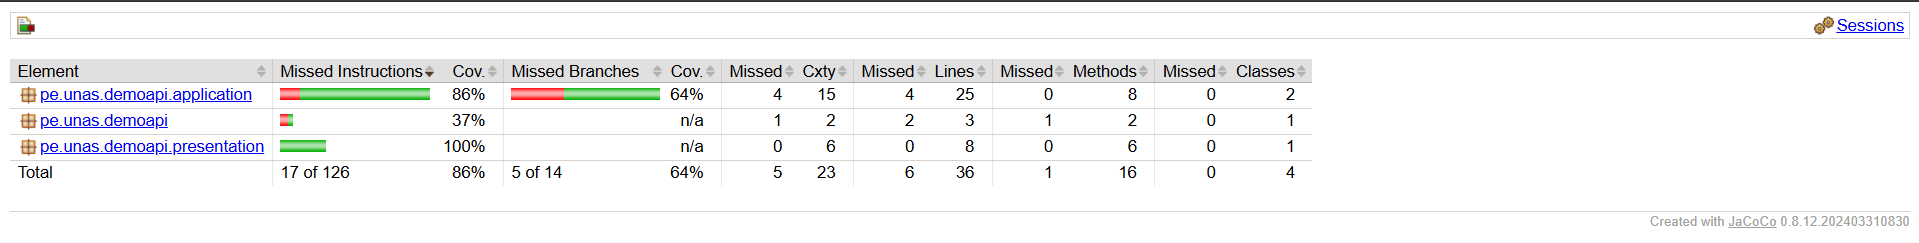
\includegraphics[width=0.8\textwidth]{image.png}
  \caption{Dimensiones del enfoque socio-tecnológico de SICOLEGIO 360}
  \label{fig:anexo_socio}
\end{figure}

% ─────────────────────────────────────────────────────────────
\chapter*{Anexo 2: Pir\'amide de Niveles Organizacionales}
\addcontentsline{toc}{chapter}{Anexo 2: Pir\'amide de Niveles Organizacionales}

\begin{figure}[H]
  \centering
  
\includegraphics[width=0.8\textwidth]{1.png}
  \caption{Pirámide de niveles Organizacionales}
  \label{fig:anexo_piramide}
\end{figure}

% ─────────────────────────────────────────────────────────────
\chapter*{Anexo 3: Tipos de Sistemas de Informaci\'on}
\addcontentsline{toc}{chapter}{Anexo 3: Tipos de Sistemas de Informaci\'on}

\begin{figure}[H]
  \centering
  
\includegraphics[width=0.8\textwidth]{3.png}
  \caption{Relación entre tipos de sistemas en SICOLEGIO 360}
  \label{fig:anexo_interaccion}
\end{figure}

\end{document}
